\documentclass[12pt,openany]{article}
\usepackage{fullpage}
\usepackage[UKenglish]{isodate}
\usepackage[colorlinks=true, linkcolor=black, citecolor=green, filecolor=magenta, urlcolor=blue]{hyperref}
\usepackage[T1]{fontenc}
\usepackage{enumitem}
\usepackage{amsmath}
\usepackage{graphicx}
\usepackage{cleveref}
\usepackage{tikz}
\usepackage{pgfplots}
\usepackage{lmodern}
\usepackage{booktabs}
\usepackage{listings}
\usepackage{amssymb}
\crefname{section}{\S\!\!}{\S}
\Crefname{section}{\S\!\!}{\S}

%% Custom colours
\definecolor{darkgreen}{rgb}{0.0, 0.42, 0.24}
\definecolor{light-gray}{gray}{0.85}
% C++ Code
\definecolor{mygreen}{rgb}{0,0.6,0}
\definecolor{mygray}{rgb}{0.5,0.5,0.5}
\definecolor{mymauve}{rgb}{0.58,0,0.82}

\usetikzlibrary{automata, positioning}

\def\CC{{C\nolinebreak[4]\hspace{-.05em}\raisebox{.4ex}{\tiny\bf ++}}}

\def\CCC{{C\nolinebreak[4]\hspace{-.05em}\raisebox{.4ex}{\small\bf ++}}}

\newcommand{\shellcmd}[1]{\\\indent\indent\texttt{\footnotesize\$ #1}}

\newcommand{\fundef}[1]{\\\indent\indent\texttt{#1}\\}

%% code listing
\lstset{ %
  backgroundcolor=\color{white},   % choose the background color; you must add \usepackage{color} or \usepackage{xcolor}
  basicstyle=\ttfamily,        % the size of the fonts that are used for the code
  %belowskip=-0.8\baselineskip,
  breakatwhitespace=false,         % sets if automatic breaks should only happen at whitespace
  breaklines=true,                 % sets automatic line breaking
  captionpos=b,                    % sets the caption-position to bottom
  commentstyle=\color{mygreen},    % comment style
  deletekeywords={...},            % if you want to delete keywords from the given language
  escapeinside={\%*}{*)},          % if you want to add LaTeX within your code
  extendedchars=true,              % lets you use non-ASCII characters; for 8-bits encodings only, does not work with UTF-8
  frame=false,                    % adds a frame around the code
  keepspaces=true,                 % keeps spaces in text, useful for keeping indentation of code (possibly needs columns=flexible)
  keywordstyle=\color{blue},       % keyword style
  language=C++,                 % the language of the code
  literate={~} {\mytilde}{1},
  morekeywords={*,...},            % if you want to add more keywords to the set
  numbers=left,                    % where to put the line-numbers; possible values are (none, left, right)
  numbersep=5pt,                   % how far the line-numbers are from the code
  numberstyle=\tiny\color{mygray}, % the style that is used for the line-numbers
  rulecolor=\color{black},         % if not set, the frame-color may be changed on line-breaks within not-black text (e.g. comments (green here))
  showspaces=false,                % show spaces everywhere adding particular underscores; it overrides 'showstringspaces'
  showstringspaces=false,          % underline spaces within strings only
  showtabs=false,                  % show tabs within strings adding particular underscores
  stepnumber=1,                    % the step between two line-numbers. If it's 1, each line will be numbered
  stringstyle=\color{mymauve},     % string literal style
  tabsize=2,                       % sets default tabsize to 2 spaces
  title=\lstname                   % show the filename of files included with \lstinputlisting; also try caption instead of title
}


\begin{document}
	\title{\bf muxstep: an open-source \CCC\ multiplex\\ HMM library for making inferences \\on multiple data types}
	\author{Petar Veli\v{c}kovi\'{c}$^*$ and Pietro Li\`{o}\\{\small Computer Laboratory, University of Cambridge, Cambridge CB3 0FD, UK}\\{\footnotesize $^*$To whom correspondence should be addressed: {\tt petar.velickovic@cl.cam.ac.uk}}}
	\date{\it Supplementary information}
	\maketitle
\tableofcontents
	\section{Introduction}
	In this document, we provide supplementary information for the applications note \emph{``{\bf muxstep}: an open source \CC\ multiplex HMM library for making inferences on multiple data types''}, for the purposes of making our work more accessible and usable to potential users. This will involve the following aspects (with section numbers):
	\begin{itemize}
		\item[{\bf \cref{sec:theory}}:] An overview of the theoretical foundations of the underlying machine learning model;
		\item[{\bf \cref{sec:install}}:] Instructions on how to properly install and use the library in new projects;
		\item[{\bf \cref{sec:format}}:] Descriptions of data formats and structures used internally by the implementation;
		\item[{\bf \cref{sec:func}}:] Thorough accounts of the functions that can be directly used when linking the library;
		\item[{\bf \cref{sec:auxx}}:] A tutorial for taking full advantage of the provided auxiliary tools;
		\item[{\bf \cref{sec:basic}}:] The basic example of using the library out-of-the-box;
		\item[{\bf \cref{sec:study}}:] An overview of a relevant case study from the authors' previous publication;
		\item[{\bf \cref{sec:mod}}:] Characteristic ways in which the library could be modified to suit specific requirements.
	\end{itemize}
	
	\subsection{Motivation}
	
	The {\bf muxstep} project is envisioned as, to the best of our knowledge, the first open-source machine learning library that integrates multiple data types simultaneously while taking advantage of the phenomenon of multiplexity, which commonly arises in a variety of natural and artificial systems. This presents a potential new scope of machine learning applications, as the learning algorithms will be able to more accurately represent patterns from a larger space of information. Furthermore, the library has been designed to be immediately usable for a large number of applications, and easily extendible for many common further use cases.\\ \\
	We focus on the common problem of \emph{binary classification}, that is, assuming the existence of two classes (often denoted as \emph{positive} and \emph{negative}), determining which class should an unseen data input belong to. In \cref{sec:kary}, we will outline ways in which the implementation can easily be extended to handle the more general case of $k$ classes.
	
	\subsection{Theoretical overview}\label{sec:theory}
	
	This subsection presents a formal specification of the model used in the implementation, in a bottom-up fashion. It mostly presents a condensed form of the material already given in the original publication by the authors \cite{Velickovic15}, where the model is described in greater detail.\\ \\ The main task that we aim to solve is classification of ordered sequences of tuples of $t$ real values, where $t$ is the number of data types being considered. Furthermore, we may attach to each tuple in the sequence a ``sub-output'' from a given discrete set of sub-outputs, $O$. For example, for $t = 2$ and $O = \{x, y, z\}$, a possible sequence to be classified is:
	\begin{equation}
		\vec{y} = \left[\left(x, \left(0.1234, 0.13849\right)\right), \left(y, \left(0.44332, 0.31849\right)\right), \left(x, \left(0.144, 0.92\right)\right)\right]
	\end{equation}
	Throughout our previous work we have assumed that these tuples can be constructed \emph{with certainty}. However, given that the model has been shown to be reasonably robust to noise on the provided data \cite{Velickovic15}, we believe that, as long as the levels of uncertainty with aligning the data are small, one may choose the most-likely alignment and still achieve good performance.
	
	\subsubsection{Single-layer GMHMM}
	
	Initially, we are interested in a way to create a model that would generate only sequences containing a {\bf single data type}. This can be modelled by a Gaussian mixture hidden Markov model (GMHMM). Informally, it is a memoryless system with $n$ possible states, which, at each time step, changes the current state it is in (according to a given distribution of transitioning probabilities), and then produces a sub-output from its new state, which then produces an output according to a Gaussian distribution (it is also possible to use other distributions---refer to \cref{sec:difdist} for implementation details).\\ \\
	The following parameters are sufficient to completely specify this model:
	\begin{itemize}
		\item The \textbf{start-state probability vector}, $\vec{\pi}$, such that $\pi_x$ specifies the probability of starting the process in state $x$;
		\item The \textbf{transition probability matrix}, $\bf T$, such that ${\bf T}_{xy}$ specifies the probability of transitioning into state $y$ from state $x$;
		\item The \textbf{sub-output probability matrix}, $\bf O$, such that ${\bf O}_{xy'}$ specifies the probability of producing sub-output $y'$ from state $x$;
		\item The \textbf{means and standard deviations} for the Gaussian distributions associated with each sub-output, $\vec{\mu}$ and $\vec{\sigma}$, such that the probability density function of the output, assuming that the sub-output is $y'$, is $\mathcal{N}(x; \mu_{y'}, \sigma_{y'}) = \frac{1}{\sqrt{2\pi\sigma_{y'}^2}}\exp\left(-\frac{(x - \mu_{y'})^2}{2\sigma_{y'}^2}\right)$.
	\end{itemize}
	An example of a GMHMM is given in Figure 1. The parameters given above can be easily learned from the training data; the output parameters $\vec{\mu}$ and $\vec{\sigma}$ are learned by computing sample means and sample standard deviations over all $(sub\_output, output)$ pairs in the training set, while the remaining parameters are derived using the standard \emph{Baum-Welch algorithm} \cite{Rabiner89}.\\ \\
	It should be noted that here, and throughout the specification, the number of nodes in the system, $n$, is problem-specific and should be {\bf manually chosen} after trying several values. While attempting to apply the model to a bioinformatics problem, we noted that smaller values (e.g. $n = 4$) should generally be more effective in capturing the properties of the system.
	
	\begin{figure}[h]
\centering 	
\begin{tikzpicture}[-stealth,very thick,node distance = 4cm,auto]

    \node[state] (x) {$x$};
    \node[state] (y) [above right of=x] {$y$};
    \node[state] (z) [below right of=y] {$z$};
    
    \node[rectangle, minimum size=2em,draw] (a) [above left =of y] {$a$};
    \node[rectangle,minimum size=2em, draw] (b) [above = of y] {$b$};
    \node[rectangle, minimum size=2em,draw] (c) [above right =of y] {$c$};

	\draw[] (x) to node[above left] {$1$} (y);
	\draw[loop above] (y) to node {$0.5$} (y);
	\draw[bend left=20] (y) to node {$0.5$} (z);
	\draw[bend left=20] (z) to node[below left] {$0.7$} (y);
	\draw[] (z) to node {$0.3$} (x);
	
	\draw[dashed] (x) to node[left] {$0.9$} (a);
	\draw[dashed] (x) to node[left] {$0.1$} (b);
	\draw[bend right=30, dashed] (y) to node[right] {$0.6$} (b);
	\draw[dashed] (y) to node[below right] {$0.4$} (c);
	\draw[dashed] (z) to node[right] {$1$} (c);
\node[rectangle, draw, scale=0.2, minimum size=20em,above = 2cm of a] (ga){\begin{tikzpicture}
\begin{axis}[axis lines=none, ticks=none,xmax=3, xmin=-3,ymax=1.1]
\addplot[ultra thick,black, no markers,samples=200] {exp(-x^2)};
\end{axis}\end{tikzpicture}};
\node[rectangle, draw, scale=0.2, minimum size=20em,above = 2cm of b] (gb){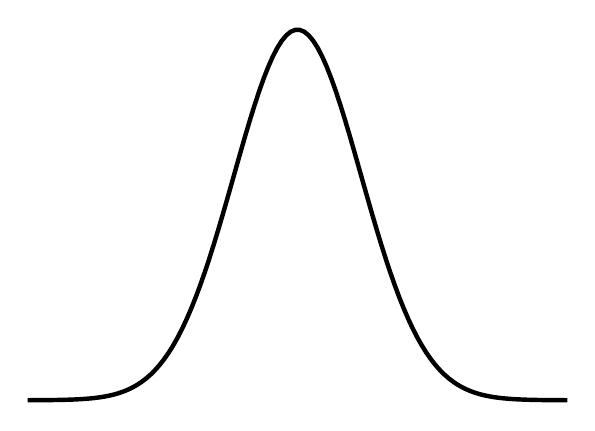
\begin{tikzpicture}
\begin{axis}[axis lines=none, ticks=none,xmax=3, xmin=-3,ymax=1.1]
\addplot[ultra thick,black, no markers,samples=200] {exp(-x^2)};
\end{axis}\end{tikzpicture}};
\node[rectangle, draw, scale=0.2, minimum size=20em,above = 2cm of c] (gc){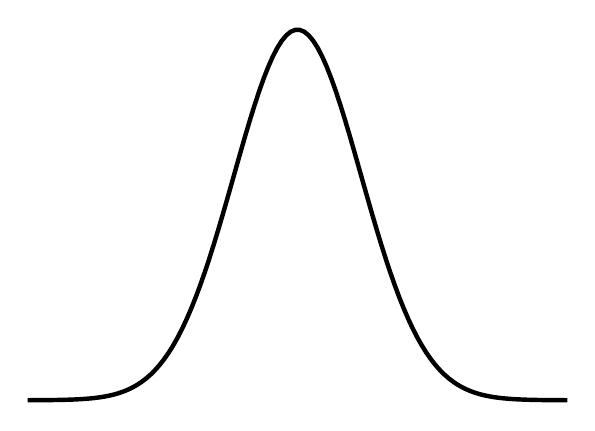
\begin{tikzpicture}
\begin{axis}[axis lines=none, ticks=none,xmax=3, xmin=-3,ymax=1.1]
\addplot[ultra thick,black, no markers,samples=200] {exp(-x^2)};
\end{axis}\end{tikzpicture}};

\draw[dotted, bend left] (a) to node[left] {$\mu_a$} (ga);
\draw[dotted, bend right] (a) to node[right] {$\sigma_a$} (ga);
\draw[dotted, bend left] (b) to node[left] {$\mu_b$} (gb);
\draw[dotted, bend right] (b) to node[right] {$\sigma_b$} (gb);
\draw[dotted, bend left] (c) to node[left] {$\mu_c$} (gc);
\draw[dotted, bend right] (c) to node[right] {$\sigma_c$} (gc);

\end{tikzpicture}
\caption[Example of a Gaussian mixture hidden Markov model]{\centering Example of a Gaussian mixture hidden Markov model, with the state set $S=\{x, y, z\}$, and sub-output set $O=\{a, b, c\}$.}\label{figgmhmm}
\end{figure}
	
	\subsubsection{Multiplex GMHMM}
	
	Once we have a model which can accurately represent sequences of a single type of data, we then extend it to handle $t$ data types simultaneously by following the steps given below, assuming that the processes interact in a multiplex nature (which holds for many real-world systems):
	\begin{enumerate}
		\item Individually train $t$ single-layer GMHMMs with $n$ nodes each, to model each of the $t$ data types separately;
		\item Then, add and train additional interlayer transitions between a node and its ``images'' in other layers;
		\item Treat the entire system as a large-scale GMHMM (after normalisation of relevant transition probabilities).
	\end{enumerate}
	In this model, we assume that the multiplex network is \emph{layer-coupled}, which means that the transition probability between a given (ordered) pair of layers is the same regardless of the current node we are in; these probabilities can then be specified by a $t \times t$ matrix, $\boldsymbol\omega$, such that ${\boldsymbol\omega}_{ij}$ specifies the probability of transitioning from layer $i$ to layer $j$.\\ \\
	This means that, within a multiplex GMHMM, the system is at each point in time in state $(x, l)$, where $x$ is a node and $l$ is a layer. It may then either change its node (but stay in the same layer), or change its layer (but stay in the same node) as specified by the transition probabilities in $\bf T$ and $\boldsymbol\omega$. When in any layer, {\bf we consider only the output Gaussian distribution corresponding to that layer}; {\it all of the other types are considered to be produced with probability 1!} More formally, the parameters of the multiplex GMHMM are as follows (assuming $(\vec{\pi}^i, {\bf T}^i, {\bf O}^i, \vec{\mu}^i, \vec{\sigma}^i)$ are the parameters of the $i$th GMHMM layer):
	\begin{equation}
	{\pi}_{(x, i)} = \boldsymbol\omega_{ii}\pi_x^i
\end{equation}
\begin{equation}
	{\bf T}_{(a, i), (b, j)} = \begin{cases}
 	0 & a\neq b \wedge i\neq j\\
 	\boldsymbol\omega_{ij} & a=b\wedge i\neq j\\
 	\boldsymbol\omega_{ii}{\bf T}_{ab}^{i} & i=j\\
 \end{cases}\end{equation}
\begin{equation}
	{\bf O}_{(x, i), y'} = 	{\bf O}_{xy'}^i
	\end{equation}
\begin{equation}
	\mu_{(y', i)} = \mu_{y'}^i
	\end{equation}
\begin{equation}
	\sigma_{(y', i)} = \sigma_{y'}^i
	\end{equation}
	The only new parameter required to specify this model is $\boldsymbol\omega$; as the exact relations between processes are typically unknown, we used an approach which makes no further assumptions about the solution space; namely, a multiobjective genetic algorithm, \emph{NSGA-II} \cite{Deb02}.\\ \\
	While we have not specifically focused on interpretation of the final model parameters obtained in prior work, it should be the case that, as with any other HMM, they should be useful for ``reverse-engineering'' the internals of the underlying processes and their interactions. Each layer is individually specialised by the well-established Baum-Welch procedure, which was already helpful in obtaining feedback on a variety of biological processes, while the entries of $\boldsymbol\omega$ could be interpreted as the \emph{relative importances} of the processes considered as relevant for the particular task; in particular we propose two interpretations of special cases:
	\begin{itemize}
		\item Two layers, $i$ and $j$, having relatively high transition probabilities ${\boldsymbol\omega}_{ij}$ and ${\boldsymbol\omega}_{ji}$, implies that their processes are heavily \emph{cooperated} in producing this issue (the system is more likely to frequently \emph{switch between them} when producing the output sequences).
		\item A layer $i$ having a relatively small probability of retention ${\boldsymbol\omega}_{ii}$, as well as small probabilities of arrival ${\boldsymbol\omega}_{xi}\ (x \neq i)$ implies that $i$'s process is likely \emph{irrelevant} for the problem specification being considered, either by true irrelevance or by being completely specified by the other feature processes considered. Such layers may then be excluded from consideration, providing further simplification to the model without sacrificing performance.
	\end{itemize}
	More complicated cases should likely be investigated in greater detail. It could be beneficial to apply the \emph{Viterbi algorithm} on a set of test sequences, to observe the states the model is most likely to go through while producing them, and draw conclusions from there (potentially with feedback from expertise).
	
	\subsubsection{Top-level classifier}
	
	Finally, in order to classify sequences based on the above models, we create \emph{two} multiplex GMHMMs; one trained to produce all the positive sequences in the training set, the other trained to produce all the negative sequences. As mentioned before, we may treat the entire multiplex GMHMM as a larger-scale GMHMM, allowing us to take advantage of the standard \emph{forward algorithm} for evaluating the likelihood that an unseen sequence was produced by that model. Classification then simply reduces to choosing the class with the higher likelihood.
	
	\subsection{Time/space complexity}
	
	We emphasise that all of the algorithms involved in the above description are computationally tractable, i.e. of time and space complexities that are polynomial in all of the input variables. In this subsection we will briefly state the relevant time and space complexities; for a detailed derivation of these complexities, refer to \cite{Velickovic15}.
	\begin{itemize}
		\item \emph{Storing the parameters} of the model with state set $S$, sub-output set $O$ and $t$ layers requires a space complexity of $O(t^2 + |S|^2\cdot t + |S|\cdot |O|\cdot t)$;
		\item The \emph{training} procedure of the multiplex GMHMM classifier has asymptotic time complexity $O(t\cdot(|S|^2 + |S|\cdot |O|)\cdot T + i\cdot p^2\cdot seq + i\cdot p\cdot(t\cdot |S|)^2\cdot T)$, and auxiliary space complexity $O(p\cdot seq + t\cdot |S|\cdot T)$, where $seq$ is the number of training sequences in the training set, $T$ is their combined length, $i$ is the number of NSGA-II iterations performed, and $p$ is the NSGA-II population size;
		\item The \emph{classification} procedure for an unseen sequence of length $\ell$ on the classifier has asymptotic time complexity $O((t\cdot |S|)^2\cdot \ell)$ and auxiliary space complexity $O(t \cdot |S|\cdot \ell)$.
	\end{itemize}
	
	\section{Installation}\label{sec:install}
	The full source code of {\bf muxstep} is hosted on the corresponding author's GitHub profile, at \url{https://github.com/PetarV-/muxstep}, and is licensed under the MIT license. The source may be downloaded as an archive from GitHub, or the repository may be directly cloned by running the following command within a terminal:
	\shellcmd{git clone https://github.com/PetarV-/muxstep.git}
	\subsection{Prerequisites}
	The muxstep library is implemented in \CC\ and is not dependent on any libraries outside of the \CC11 standard template library. In order to build the library from source (or link it against other \CC\ code), {\tt clang++} is required; on Mac OS X, this compiler is installed by default.
	\subsection{Compilation}
	Compiling the libraries is extremely simple; in any terminal, while in the root directory of the repository, simply run
	\shellcmd{make}\\
	after which the libraries (both static and dynamic) will be created in the {\tt lib/} folder.
	\subsection{Linking}
	In order to use the library implementations within your own projects, you need to first {\tt \#include} the relevant header files in your project (normally, only {\tt \#include <classifier.h>} is necessary; \cref{sec:func} will explain what is exposed by each header in more detail).\\ \\
	Then, to link your project with the static library, you need to compile it like so:
	\shellcmd{clang++ -std=c++11 -Ipath/to/include file.cpp -Lpath/to/lib -lmuxstep -o app}\\
	where:
	\begin{itemize}
		\item {\tt file.cpp} is the name of your project file(s);
		\item {\tt path/to/include} is the (relative) path to the folder containing the {\tt .h} files;
		\item {\tt path/to/lib} is the (relative) path to the folder containing the static library;
		\item {\tt app} is the name of the compiled executable.
	\end{itemize}
	After this, you may launch your executable by simply running
	\shellcmd{./app}\\ \\
	If, instead, you would like to link with the dynamic library, you need to execute the following sequence of commands:
	\shellcmd{clang++ -std=c++11 -Ipath/to/include file.cpp -Lpath/to/lib -lmuxstep.dyn -o app}
	\shellcmd{LD\_LIBRARY\_PATH=\$LD\_LIBRARY\_PATH:/path/to/muxstep/lib/}
	\shellcmd{export LD\_LIBRARY\_PATH}\\
	where {\tt /path/to/multiplex/lib} is the absolute path to the folder containing the dynamic library, and everything else is the same as before.
	\section{Internal data formats and structures}\label{sec:format}
	\subsection{Model parameters format}
	A common action one might wish to do is store model parameters for later use. To accommodate this, we have overloaded the standard \CC\ stream operators ({\tt >\/>}, {\tt <\/<}) in order to directly read to/write from a pointer to a classifier. The format in which this data is moved around is as follows:
	\begin{itemize}
		\item The first line contains three integers, $n$, $s$ and $t$, representing the number of nodes in each layer, the number of sub-outputs, and the number of data types ($\sim$ layers) considered, respectively.
		\item Afterwards, the positive and negative multiplex GMHMMs are specified in that order; a single multiplex GMHMM is represented as follows:
		\begin{itemize}
			\item The first line contains three integers, $n$, $s$ and $t$, with the same meaning as before.
			\item Afterwards, each of the $t$ GMHMM layers are represented, in order, as follows:
			\begin{itemize}
				\item The first line contains two integers, $n$ and $s$, with the same meaning as before.
				\item The second line contains $n$ real numbers, representing the vector $\vec{\pi}$.
				\item The next $n$ lines each contain $n$ real numbers, representing the entries of the matrix $\bf T$.
				\item The next $n$ lines each contain $s$ real numbers, representing the entries of the matrix $\bf O$.
				\item The remaining lines contain the representation of the output probability distribution. If the Gaussian distribution is used (default):
					\begin{itemize}
					\item The first line will contain $s$;
					\item The next $s$ lines each contain two real numbers, representing the $\mu$ and $\sigma$ values for each sub-output.
					\end{itemize}
			\end{itemize}
			\item Afterwards, the next $t$ lines each contain $t$ real numbers, representing the entries of the matrix $\boldsymbol\omega$.
		\end{itemize}
	\end{itemize}
	The format as described contains several redundancies, but this is introduced for the purpose of making recursive input/output of the entire model as simple as possible.
	\subsection{Data structures for training parameters}\label{sec:trnparam}
	The training subroutines used within the model training (namely, the \emph{Baum-Welch algorithm} and \emph{NSGA-II}) are both relying on specific parameters in order to, for example, determine the desirable level of convergence, or the maximal number of iterations. It could potentially be useful to fine-tune these parameters in order to obtain, for example, faster training times at the expense of precision.\\ \\
	These parameters are declared within two {\tt struct}s, {\tt nsga2\_params} and {\tt baumwelch\_params}, which have to be passed to the {\tt MultiplexGMHMMClassifier} class when constructing it.\\ \\
	The {\tt baumwelch\_params} {\tt struct} is very simple and contains only two variables, {\tt iterations} and {\tt tolerance}, signifying that the Baum-Welch algorithm should be executed until either executing {\tt iterations} steps, or reaching convergence on the level up to {\tt tolerance}.\\ \\
	We now turn our attention to the more complicated {\tt nsga2\_params} {\tt struct}. It contains the following values:
	\begin{itemize}
		\item[\tt pop\_size:] population size;
		\item[\tt ft\_size:] number of features (determined by the number of data types $t$, as $t \cdot t$);
		\item[\tt obj\_size:] number of objectives (equal to the size of the training set);
		\item[\tt generations:] number of generations to iterate over;
		\item[\tt p\_crossover:] crossover probability;
		\item[\tt p\_mutation:] mutation probability;
		\item[\tt di\_crossover:] crossover distribution index;
		\item[\tt di\_mutation:] mutation distribution index;
		\item[\tt var\_lims:] a {\tt vector} of size {\tt ft\_size}, consisting of {\tt pair}s of {\tt double}s specifying the lower and upper bounds on each of the features' values.
	\end{itemize}
	Finally, we recommend a key-value format of specifying these parameters, as can be seen in {\tt examples/training\_params.in}. The basic usage example (discussed in \cref{sec:basic}) also contains a function for parsing a file in this format.
	\subsection{Data structure for input sequences}
	Looking back to Equation 1, we have decided to represent a single input sequence as the following \CC\ data structure:
	\begin{center}
		{\tt vector<pair<int, vector<double> > >}
	\end{center}
	This represents a vector of data points, where each data point is actually a pair of a sub-output (represented by an integer) and a vector of the $t$ data types at that data point. The data points should be ordered in some way; if they represent snapshots in time, then this is already a natural ordering; otherwise, a sorting procedure could be employed to them first, before giving them to the model for processing.\\ \\
	Following from there, the training procedure will expect a vector of labeled sequences, represented as:
	\begin{center}
		{\tt vector<pair<\underline{\ttfamily \fontseries{b}\selectfont vector<pair<int, vector<double> > >}, bool> >}
	\end{center}
	The underlined part here represents a single sequence as given above, for clarity. Each sequence is paired up with its label (true/false $\sim$ positive/negative).
	
	\section{Exposed functions}\label{sec:func}
	This section will present the functions exposed by each of the header files within the {\tt include/} directory. Functions of particular interest for {\bf \textcolor{blue}{essential usage}} will be highlighted with a {\bf \textcolor{blue}{blue}} colour, while functions of particular interest for {\bf \textcolor{red}{modifying and extending the library}} will be highlighted with a {\bf \textcolor{red}{red}} colour.
	\subsection{\tt distribution.h}\label{sec:disthdr}
	\hfill\vspace*{-10pt}\fundef{virtual Distribution::\textasciitilde Distribution()}
	\emph{Abstract destructor}.
	\fundef{virtual Distribution::clone()}
	\emph{Abstract function}; returns a clone of a given distribution.
	\textcolor{red}{\fundef{virtual Distribution::train(train\_set)}}
	\emph{Abstract function}; trains the distribution parameters using the data in {\tt train\_set}.
	\textcolor{red}{\fundef{virtual Distribution::get\_probability(obs\_id, x)}}
	\emph{Abstract function}; returns the probability of producing output {\tt x}, under the assumption that the current sub-output is {\tt obs\_id}.
	\fundef{virtual Distribution::read(in)}
	\emph{Abstract function}; reads into a distribution from the input stream {\tt in}.
	\fundef{virtual Distribution::write(out)}
	\emph{Abstract function}; writes a distribution through the output stream {\tt out}.\\ \\
	A particular example of a class implementing this interface is the {\tt Gaussian} class, defined in {\tt include/gaussian.h} and implemented in {\tt src/gmhmm/gaussian.cpp}.
	
	\subsection{\tt gmhmm.h}
	
	\hfill\vspace*{-10pt}\fundef{GMHMM::GMHMM(n, obs)}
	Constructor; creates a random GMHMM with {\tt n} nodes and {\tt obs} sub-outputs.
	\fundef{GMHMM::GMHMM(n, obs, pi, T, O, mu, sigma)}
	Constructor; creates a known GMHMM from its parameters.
	\fundef{GMHMM::GMHMM(n, obs, pi, T, O, d)}
	Constructor; creates a known MHMM with a custom distribution {\tt d}.
	\fundef{GMHMM::GMHMM(gmhmm)}
	Constructor; copies a known GMHMM.
	\fundef{GMHMM::\textasciitilde GMHMM()}
	Destructor; clears all resources used.
	\fundef{GMHMM::forward(Y)}
	Implementation of the \emph{forward algorithm} on sequence {\tt Y}.
	\fundef{GMHMM::backward(Y, c)}
	Implementation of the \emph{backward algorithm} on sequence {\tt Y} and scaling coefficients {\tt c}.
	\fundef{GMHMM::baumwelch(Ys, iterations, tolerance)}
	Implementation of the \emph{Baum-Welch algorithm} on the sequence set {\tt Ys}.\\
	Runs until convergence (specified by {\tt tolerance}), or until {\tt iterations} steps are performed.
	\fundef{GMHMM::get\_pi(x)}
	Getter; returns $\pi_{\tt x}$.
	\fundef{GMHMM::get\_T(i, j)}
	Getter; returns ${\bf T}_{\tt ij}$.
	\fundef{GMHMM::get\_O(x, y)}
	Getter; returns ${\bf O}_{\tt xy}$.
	\fundef{GMHMM::get\_D()}
	Getter; returns the probability distribution used by this (G)MHMM.
	\textcolor{red}{\fundef{GMHMM::train(train\_set, params)}}
	Trains the model parameters using the data in {\tt train\_set}, using the parameters in {\tt params} for the Baum-Welch algorithm.
	\fundef{GMHMM::log\_likelihood(test\_data)}
	Returns the likelihood of producing the sequence {\tt test\_data} by the model.
	\fundef{operator>\/>(in, G)}
	Reads a GMHMM into {\tt G} from the input stream {\tt in}.
	\fundef{operator<\/<(out, G)}
	Writes the GMHMM {\tt G} through the output stream {\tt out}.
	
	\subsection{\tt multiplex\_gmhmm.h}
	\hfill\vspace*{-10pt}\fundef{MultiplexGMHMM::MultiplexGMHMM(n, obs, L)}
	Constructor; creates a random multiplex GMHMM with {\tt n} nodes, {\tt obs} sub-outputs and {\tt L} layers ($\sim$ data types).
	\fundef{MultiplexGMHMM::MultiplexGMHMM(n, obs, L, layers, omega)}
	Constructor; creates a known multiplex GMHMM from its parameters.
	\fundef{MultiplexGMHMM::MultiplexGMHMM(m\_gmhmm)}
	Constructor; copies a known multiplex GMHMM.	
	\fundef{MultiplexGMHMM::\textasciitilde MultiplexGMHMM()}
	Destructor; clears all resources used.
	\fundef{MultiplexGMHMM::set\_omega(omega)}
	Setter; sets the matrix $\boldsymbol\omega$ to the values in {\tt omega} and normalises all transition probabilities.
	\textcolor{red}{\fundef{MultiplexGMHMM::train(train\_set, nsga\_p, bw\_p)}}
	Trains the model parameters using the data in {\tt train\_set}, using the parameters in {\tt nsga\_p} for NSGA-II and the parameters in {\tt bw\_p} for the Baum-Welch algorithm.
	\fundef{MultiplexGMHMM::log\_likelihood(test\_data)}
	Returns the likelihood of producing the sequence {\tt test\_data} by the model.
	\fundef{operator>\/>(in, M)}
	Reads a multiplex GMHMM into {\tt M} from the input stream {\tt in}.
	\fundef{operator<\/<(out, M)}
	Writes the multiplex GMHMM {\tt M} through the output stream {\tt out}.
		
	\subsection{\tt classifier.h}\label{sec:classhdr}
	
	\hfill\vspace*{-10pt}\fundef{\textcolor{blue}{MultiplexGMHMMClassifier::MultiplexGMHMMClassifier(node\_count, sub\_count,}}\vspace*{-15pt}\fundef{\textcolor{blue}{type\_count, nsga\_p, bw\_p)}}
	Constructor; creates a random multiplex GMHMM classifier with {\tt node\_count} nodes, {\tt sub\_count} sub-outputs and {\tt type\_count} layers ($\sim$ data types). Also stores the parameters in {\tt nsga\_p} and {\tt bw\_p} for later use during training.
	\fundef{MultiplexGMHMMClassifier::MultiplexGMHMMClassifier(node\_count, sub\_count,}\vspace*{-15pt}\fundef{type\_count, nsga\_p, bw\_p, positive, negative)}
	Constructor; creates a known multiplex GMHMM classifier from its parameters.
	\fundef{MultiplexGMHMMClassifier::\textasciitilde MultiplexGMHMMClassifier()}
	Destructor; clears all resources used.
	\fundef{MultiplexGMHMMClassifier::clone()}
	Returns a clone of a given multiplex GMHMM classifier.
	\fundef{\textcolor{blue}{MultiplexGMHMMClassifier::train(training\_set)}}
	Trains the model parameters using the data in {\tt training\_set}.
	\fundef{\textcolor{blue}{MultiplexGMHMMClassifier::classify(test\_data)}}
	Determines the class for the sequence {\tt test\_data}.
	\fundef{\textcolor{blue}{MultiplexGMHMMClassifier::classify\_reliable(test\_data, min\_margin)}}
	Determines the class for the sequence {\tt test\_data}, reporting whether the margin between the two classes' likelihoods is greater than {\tt min\_margin}.
	\fundef{\textcolor{blue}{operator>\/>(in, C)}}
	Reads a multiplex GMHMM classifier into {\tt C} from the input stream {\tt in}.
	\fundef{\textcolor{blue}{operator<\/<(out, C)}}
	Writes the multiplex GMHMM classifier {\tt C} through the output stream {\tt out}.
	
	\section{Auxiliary tools}\label{sec:auxx}
	For the users' convenience we have provided two tools alongside the main library, which may be useful for verifying that the model works as expected. The tools may be found in the {\tt test/} folder of the repository, and this section describes some of the ways to take advantage of them.
	\subsection{Synthetic data generator ({\tt syn\_gen})}
	The first tool we consider, called {\tt syn\_gen} for short, is used for generating synthetic sequences with data points produced according to Gaussian distributions. After compiling it (by running {\tt make} while in the {\tt test/syn\_gen} folder) you may launch the command line tool. The parameters passed to it are as follows:
	\shellcmd{./syn\_gen <input\_parameters> <output\_file> <sort?\! [Y/N]>}\\
	where:
	\begin{itemize}
		\item {\tt <input\_parameters>} represents a path to a file specifying the parameters of the sequences to be generated (more details on its format later in this section).
		\item {\tt <output\_file>} represents a path to the file which will contain the sequences' data. A file in this format (called the {\tt syn\_gen} format) can then be processed by the function provided in the basic usage example (more details on the format later in this section).
		\item {\tt <sort?>} is a boolean parameter (accepts only {\tt 'Y'} and {\tt 'N'}) that specifies whether or not the sequence should be sorted before being returned (appropriate if we are not observing our sequences through time). The metric used for sorting is the (squared) \emph{euclidean norm} of the data types; this can be easily modified in the {\tt syn\_gen.cpp} file.
	\end{itemize} 
	\subsubsection{Parameters file format}
	An example parameters file may be found in {\tt test/syn\_gen/example\_parameters}. Its format is as follows:
	\begin{itemize}
		\item The first line contains four integers: $tests$, $l$ $s$, $t$, representing:
		\begin{itemize}
			\item[$tests$:] the number of sequences of each label to generate (so for binary classification, $2\cdot tests$ sequences will be produced).
			\item[$l$:] the number of labels (for binary classification, $l = 2$).
			\item[$s$:] the number of sub-outputs.
			\item[$t$:] the number of data types ($\sim$ layers).
		\end{itemize}
		\item The second line contains two integers: $lo$, $hi$, signifying that all sequences will be of lengths $\ell \in [lo, hi]$ (drawn uniformly at random for each sequence).
		\item Afterwards, each label is specified in turn as follows:
		\begin{itemize}
			\item The first line will contain a string, the label's identifier (typically, {\tt positive} and {\tt negative} are used).
			\item Afterwards, each data type's distributions (for the current label) are specified in $s$ lines (therefore, there will be $t \cdot s$ lines in total); each of them contains two real numbers $\mu$ and $\sigma$, such that the $i$th line contains the mean and standard deviation for the Gaussian distribution of the current data type, assuming that the sub-output is $i$.
		\end{itemize}
	\end{itemize}
	\subsubsection{Output ({\tt syn\_gen}) format}
	Example outputs of {\tt syn\_gen} may be found in the {\tt example/} folder. This format is made to be easily decodable (a function for decoding it is provided in the basic example), as well as directly human-readable; as such, we recommend it as a potential format to use for storing the training and testing data. The format is defined as follows:
	\begin{itemize}
		\item The first line contains an integer $seq$, the total number of sequences in the file.
		\item The second line contains two integers $s$ and $t$, specifying the number of sub-outputs and types, respectively.
		\item Afterwards, each of the $seq$ sequences are specified (and separated by a blank line from one another), as follows:
		\begin{itemize}
			\item The first line contains a string $lab$ and an integer $len$, specifying this sequence's label and its length.
			\item The following $len$ lines each contain an integer followed by $t$ real numbers, specifying the data points of the sequence in order; each data point is represented by first the sub-output, then the $t$ data types.
		\end{itemize}
	\end{itemize}
	\subsection{Evaluation suite}
	In order to make evaluation data generation easier, we have also provided an evaluation suite which takes a file containing labelled data, and then evaluates the model on it using crossvalidation. It can be compiled by running {\tt make} while in the {\tt test/classifier} folder; this will produce a {\tt simple\_tester} executable, which can be launched as follows:
	\shellcmd{./simple\_tester <node\_count> <data\_set\_file> <training\_params\_file>}\\
	The first parameter is an integer $n$, specifying the number of nodes the model should have in each layer (we recommend running multiple tests with different values of this parameter until one is found that models the problem best), the second parameter is a path to a file in {\tt syn\_gen} format, representing the set of labelled sequences (\textbf{the labels used must be {\tt positive} and {\tt negative}!}), and the third parameter is a path to the training parameters file in the recommended format mentioned in \cref{sec:trnparam}.\\ \\
	After execution, the program will generate a separate file containing each of the crossvalidation run results, as well as a ``full'' result obtained by averaging the individual runs. The metrics computed include: \emph{accuracy}, \emph{precision}, \emph{sensitivity}, \emph{specificity}, \emph{false positive rate}, \emph{negative predictive value}, \emph{false discovery rate}, \emph{Matthews Correlation Coefficient (MCC)}, \emph{$F_1$ score}, as well as the parameters required to draw a \emph{Receiver operating characteristic (ROC) curve}.\\ \\
	A slightly more advanced use case for the evaluation suite involves \emph{evaluating the robustness of the model in the presence of noise}. To help with this, additional parameters may be passed to {\tt simple\_tester}, specifying the ranges of (Gaussian) noise means and standard deviations to evaluate the model on. For example, if we want to evaluate the model performance on all noise means between $0$ and $1$ with increments of $0.1$ and all noise standard deviations between $0$ and $2$ with increments of $0.2$, the command should be ran as follows:
	\shellcmd{./simple\_tester <node\_count> <data\_set\_file> <training\_params\_file> 0:0.1:1 0:0.2:2}
	\section{Use cases}
	\subsection{Basic usage example}\label{sec:basic}
	A basic example detailing the most common usage case of the library can be found in the {\tt example/} folder. Instructions for compiling it can be found in the repository's {\tt README} file.\\ \\ 
	The example's source code (given in {\tt basic\_usage.cpp}) initially provides two helper methods: {\tt extract\_data}, for extracting all the important information ($s$, $t$, and the data) from a {\tt syn\_gen}-formatted file and {\tt extract\_parameters}, for parsing the training parameters from a file in the recommended format from \cref{sec:trnparam}. The main function is detailedly commented and should be sufficient on its own to understand the principal elements of the workflow; therefore its detailed description is omitted from this material.\\ \\
	{\bf N.B.} The training method involved will converge to different local optima for different initial conditions, which are randomised every time the training subroutine is executed. Therefore, for general usage it is probably better to train the model several times, and choose the parameters that perform the best.
	\subsection{Worked case study}\label{sec:study}
	For the purposes of emphasising the model's potentials, and in particular that it should be applicable to virtually any kind of sortable sequences of data tuples (not restricted to temporal data), we provide an overview of a full worked case study, presented in greater detail within our original publication detailing the theoretical foundations of this model \cite{Velickovic15}.\\ \\
	We have used the model (from a pre-release version of the {\bf muxstep} library) for classifying patients for \emph{breast invasive carcinoma} (BRCA) by simultaneously considering the \emph{gene expression} and \emph{methylation} metrics of 26 genes in the tumour necrosis factor receptor superfamily (TNFRSF). The genes within a single patient sequence were ordered by a simple activity measure, namely by the euclidean norm of the two:
\begin{equation}
	activity_g = \sqrt{expression_g^2 + methylation_g^2}	
\end{equation}
The genes were considered as the sub-outputs in the model, while the $(expression, methylation)$ tuple was considered as a single data point. The model was trained and tested using data obtained from the \emph{Cancer Genome Atlas} (TCGA) containing gene expression and methylation measurements for 776 positive and 79 negative sequences. The model achieved a mean accuracy of {\bf 94.2\%}, sensitivity of {\bf 95.8\%} and $\text{F}_1$ score of {\bf 0.966} after 10-fold crossvalidation, without any effort to optimise the parameters of the training algorithm, and outperformed its single-layer counterpart on the same data set.\\ \\
The results should hopefully demonstrate that, not only is temporal ordering not required for taking advantage of this model, one does not even need a particularly ``informed'' notion of ordering a sequence.
	\subsection{Modifying the library}\label{sec:mod}
	This section lists several common ways in which the library might be modified to suit different modelling needs. The library was designed such that most of the modifications should be fairly simple to do, and some do not even require modifying/recompiling the source code.
	\subsubsection{Removing sub-outputs}
	If the sub-output layer is unnecessary for modelling the problem, a very simple way to ``eliminate'' it is to set $s = 1$ and have all data points producing sub-output $0$. That way, there will still be one explicit sub-output, but it will have no effect on the classification.
	\subsubsection{Using different output distributions}\label{sec:difdist}
	In the event that distributions other than Gaussian are more appropriate for any of the individual GMHMM layers, it is possible to provide an implementation of another distribution that should be used (extending the {\tt Distribution} abstract class as specified in \cref{sec:disthdr}. A pointer to this distribution should then be passed as a parameter while constructing the (G)MHMM.\\ \\
	The methods {\tt clone}, {\tt read} and {\tt write} should be easily implementable, and are required only to ensure that models using this distribution can still be uniquely written to a file for later use. The crucial two methods to implement are {\tt train}, which infers the distribution's parameters based on the given training set, and {\tt get\_probability}, that, given a sub-output and an output, returns the probability of producing the output assuming the sub-output. For continuous random variables, this is just the probability density function.\\ \\
	As the default option, and to serve as a reference implementation, we provide the {\tt Gaussian} class (implementation found in {\tt src/gmhmm/gaussian.cpp}). In this case, {\tt train} reduces to estimating the sample means $\vec{\mu}$ and standard deviations $\vec{\sigma}$ for each sub-output, while {\tt get\_probability} reduces to computing $\mathcal{N}(x; \mu_s, \sigma_s)$ for input $x$ and sub-output $s$.
	\subsubsection{Confidence intervals on output sequence likelihoods}
	It may be argued that using the {\tt classify\_reliable} method from \cref{sec:classhdr} takes a relatively na\"{i}ve approach to asserting reliability of the obtained labelling. A more natural approach to this could involve computing \emph{p\% confidence intervals} over the obtained class likelihoods $\mathbb{P}(\vec{y}|C_i)$ and checking for overlap with the selected class' interval.\\ \\
	A subroutine for evaluating confidence intervals has been omitted from the main library implementation as it does not fall into the needs of the usual use case of the library, and, as we will discuss below, doing it incurs a potentially unnecessary penalty in either time or space complexities. However, it should be easy to extend the library to accommodate for such computations---we provide a brief overview in this subsection.\\ \\
	In order to be able to construct a confidence interval around the likelihood, we need several samples of it derived from \emph{different models}. After this, one may apply standard statistical methods for estimating confidence intervals from these samples, and report the mean value of the samples along with the interval. An approach we suggest for doing this is to create and store a fixed number of \emph{copies} of the Multiplex GMHMM model for a particular class, all trained on the same training set, but with different (randomised) initial conditions; so that they may converge to different models. When a likelihood with a confidence interval is required for a new output sequence, one should first compute the likelihoods of producing it for each of the stored copies, and then performing the aforementioned statistical analysis on these likelihoods.\\ \\
	The approach described here incurs a constant factor (exactly equal to the number of copies being stored) cost of time and space to all of the relevant subroutines---however, we note that the time costs could be mitigated by exploiting the fact that training and classification over a single copy is independent of the others, so all of the individual {\tt train}/{\tt log\_likelihood} calls can be freely scheduled to run in parallel.
	\subsubsection{Switching to $k$-ary classification}\label{sec:kary}
	Finally, we conclude that the decision to use binary classification was made just so evaluation metrics could be more easily extracted, and because it is a common problem for which larger sources of data are available. However, the model and its inference algorithms are fully extensible to $k$-ary classification. In this case, one should train $k$ different models (one for each label), evaluate the individual probabilities of producing a new sequence, and choose the class with the highest one.\\ \\
	This requires several (relatively simple) modification steps:
	\begin{itemize}
		\item In the classifier's specification in {\tt include/classifier.h}, one needs to include a {\tt vector<MultiplexGMHMM*>}, rather than the currently used two {\tt MultiplexGMHMM*}s for the positive and negative models.
		\item The labels on the training data can now go beyond $0$ and $1$, so the type of the labels is no longer {\tt bool}, but rather an integer type, e.g. {\tt int}.
		\item Finally, the methods within {\tt src/classifier/classifier\_multiplex\_gmhmm.cpp} will need to be modified to accommodate this change (in most cases, the change is trivial).
	\end{itemize}
	In order to demonstrate how this could potentially be done, we included a new, experimental (untested) class called {\tt MultiplexKClassifier}, implementing a basic $k$-ary classifier using the steps above. This class is defined in {\tt include/classifier.h} and implemented in {\tt src/classifier/classifier\_k\_ary.cpp}.\\ \\
	Similarly to the analysis from the previous subsection, performing $k$-ary classification clearly incurs a constant factor penalty of $k$ to both the time and space complexities of the relevant subroutines. Once again, training and obtaining likelihoods for each of the models are independent operations, and therefore all calls to {\tt train}/{\tt log\_likelihood} can be executed in parallel, which should mitigate the time costs on a multi-core machine.
	\addcontentsline{toc}{section}{References}
	\begin{thebibliography}{9}
\bibitem{Deb02} Deb, K., Pratap, A., Agarwal, S., \& Meyarivan, T. A. M. T. (2002). A fast and elitist multiobjective genetic algorithm: NSGA-II. \emph{Evolutionary Computation, IEEE Transactions on, 6}(2), 182-197.
\bibitem{Rabiner89} Rabiner, L. R. (1989). A tutorial on hidden Markov models and selected applications in speech recognition. \emph{Proceedings of the IEEE}, 77(2), 257-286.
\bibitem{Velickovic15} Veli\v{c}kovi\'{c}, P., \& Li\`{o}, P. (2015). Molecular multiplex network inference using Gaussian mixture hidden Markov models. \emph{Journal of Complex Networks}, cnv029.
\end{thebibliography}
	
\end{document}
